\documentclass[pdftex,12pt,a4paper]{article}
\pdfpagewidth 8.5in
\pdfpageheight 11.6in
\linespread{1.3}
\usepackage{anysize}
\marginsize{2.5cm}{2.5cm}{2.5cm}{2.5cm}

\usepackage[utf8]{inputenc}
\usepackage[T1]{fontenc}
\usepackage[magyar]{babel}
\usepackage{indentfirst}
\usepackage{amsmath}
\usepackage{float}
\usepackage{graphicx}
\usepackage{braket}
\usepackage[unicode,pdftex]{hyperref}
%\usepackage{hyperref}
\usepackage{breqn}

\usepackage{listings}
\usepackage{xcolor}

\definecolor{codegreen}{rgb}{0,0.6,0}
\definecolor{codegray}{rgb}{0.3,0.3,0.3}
\definecolor{codepurple}{rgb}{0.58,0,0.82}
\definecolor{backcolour}{rgb}{0.90,0.90,0.87}

\lstdefinestyle{mystyle}{
    backgroundcolor=\color{backcolour},   
    commentstyle=\color{codegreen},
    keywordstyle=\color{magenta},
    numberstyle=\small\color{codegray},
    stringstyle=\color{codepurple},
    basicstyle=\ttfamily\small,
    breakatwhitespace=false,         
    breaklines=true,                 
    captionpos=b,                    
    keepspaces=true,                 
    numbers=left,                    
    numbersep=5pt,                  
    showspaces=false,                
    showstringspaces=false,
    showtabs=false,                  
    tabsize=2
}
\lstset{style=mystyle}

\DeclareMathOperator{\Ai}{Ai}
\DeclareMathOperator{\Bi}{Bi}
\DeclareMathOperator{\Aip}{Ai^\prime}
\DeclareMathOperator{\Bip}{Bi^\prime}
\DeclareMathOperator{\Ti}{Ti}
\DeclareMathOperator{\ctg}{ctg}
\DeclareMathOperator{\sgn}{sgn}
%\DeclareMathOperator{\max}{max}
\let\Im\relax
\DeclareMathOperator{\Im}{Im}
\DeclareMathOperator{\Tr}{Tr}
\newcommand{\op}[1]{\hat{#1}}
\newcommand{\norm}[1]{\left\lVert #1 \right\rVert}
\newcommand*\Laplace{\mathop{}\!\mathbin\bigtriangleup}

\newcommand{\aeqref}[1]{\az{\eqref{#1}}}
\newcommand{\Aeqref}[1]{\Az{\eqref{#1}}}

\hypersetup{
    colorlinks,
    citecolor=black,
    filecolor=black,
    linkcolor=black,
    urlcolor=black
}
\hypersetup{	
	pdftitle={Transzmissziós elektronmikroszkópia},
	pdfauthor={Kürti Zoltán}}

\frenchspacing
\begin{document}

	\centerline{\bf\LARGE Transzmissziós elektronmikroszkópia}

	\vskip0.4truein\centerline{\Large\sc Kürti Zoltán}\vskip0.10truein
	%\centerline{\includegraphics[scale=0.5]{./elte_cimer_color.pdf}}
	\vskip0.4truein
	\centerline{\Large B csoport}\vskip0.2truein
	\centerline{\Large{Mérés dátuma: 2021. november 25}}\vskip0.2truein
	\centerline{\Large{Beadás dátuma: \today}}\vskip0.2truein
	\thispagestyle{empty}
	\newpage
	%\tableofcontents
	%\newpage
	\section{Bevezetés}
		A mérés kiértékelésének nagy részét a BSc. TEM laborhoz írt programommal végeztem. Annyi a különbség, hogy a program mostani verziója használja a nagy energiás közelítést. Ez nem változtat az eredményen, viszont mivel most nem mi készítettük a képeket, a használt elektronok energiáját csak feltételezni tudnám előző mérések alapján. A kódot elküldöm pdf illetve futtatható formában is.
		
		A mikroszkóp állandó kalibrálásához nikkel porról készült diffrakciós ábrát használtunk. A cél egy szilíciumból és gallium-nitridből álló rendszer vizsgálata, a szomszédos kristályok orientációjának meghatározása.
	\section{Kalibrálás}
		\begin{figure}[H]
			\centering
			A programmal először a nikkel minta középső pontját határoztam meg. Ez után a középpontól mért távolság függvényében kiszámítottam a körvonalak mentén mért intenzitást. Ebből az intenzitásból megpróbáltam leválasztani a hátteret egy Cauchy-függvény illesztésével. Ez a lépés nem olyan fontos, e nélkül is hasonló értéket kapok a mikroszkóp állandóra. Ezek után a mikroszkóp állandót úgy optimalizálom, hogy a nikkel $d_{hkl}$ távolságai alapján várt gyűrűk helyén az intenzitások szorzata maximális legyen. \Aref{sugarak}. ábra mutatja az illesztés eredményét, valamint \aref{gyuruk}. ábra mutatja az illesztett gyűrűket a nikkel eredeti diffrakciós ábráján. $\lambda L = 367\text{pixel\AA}$ a mért mikroszkóp állandó. 
			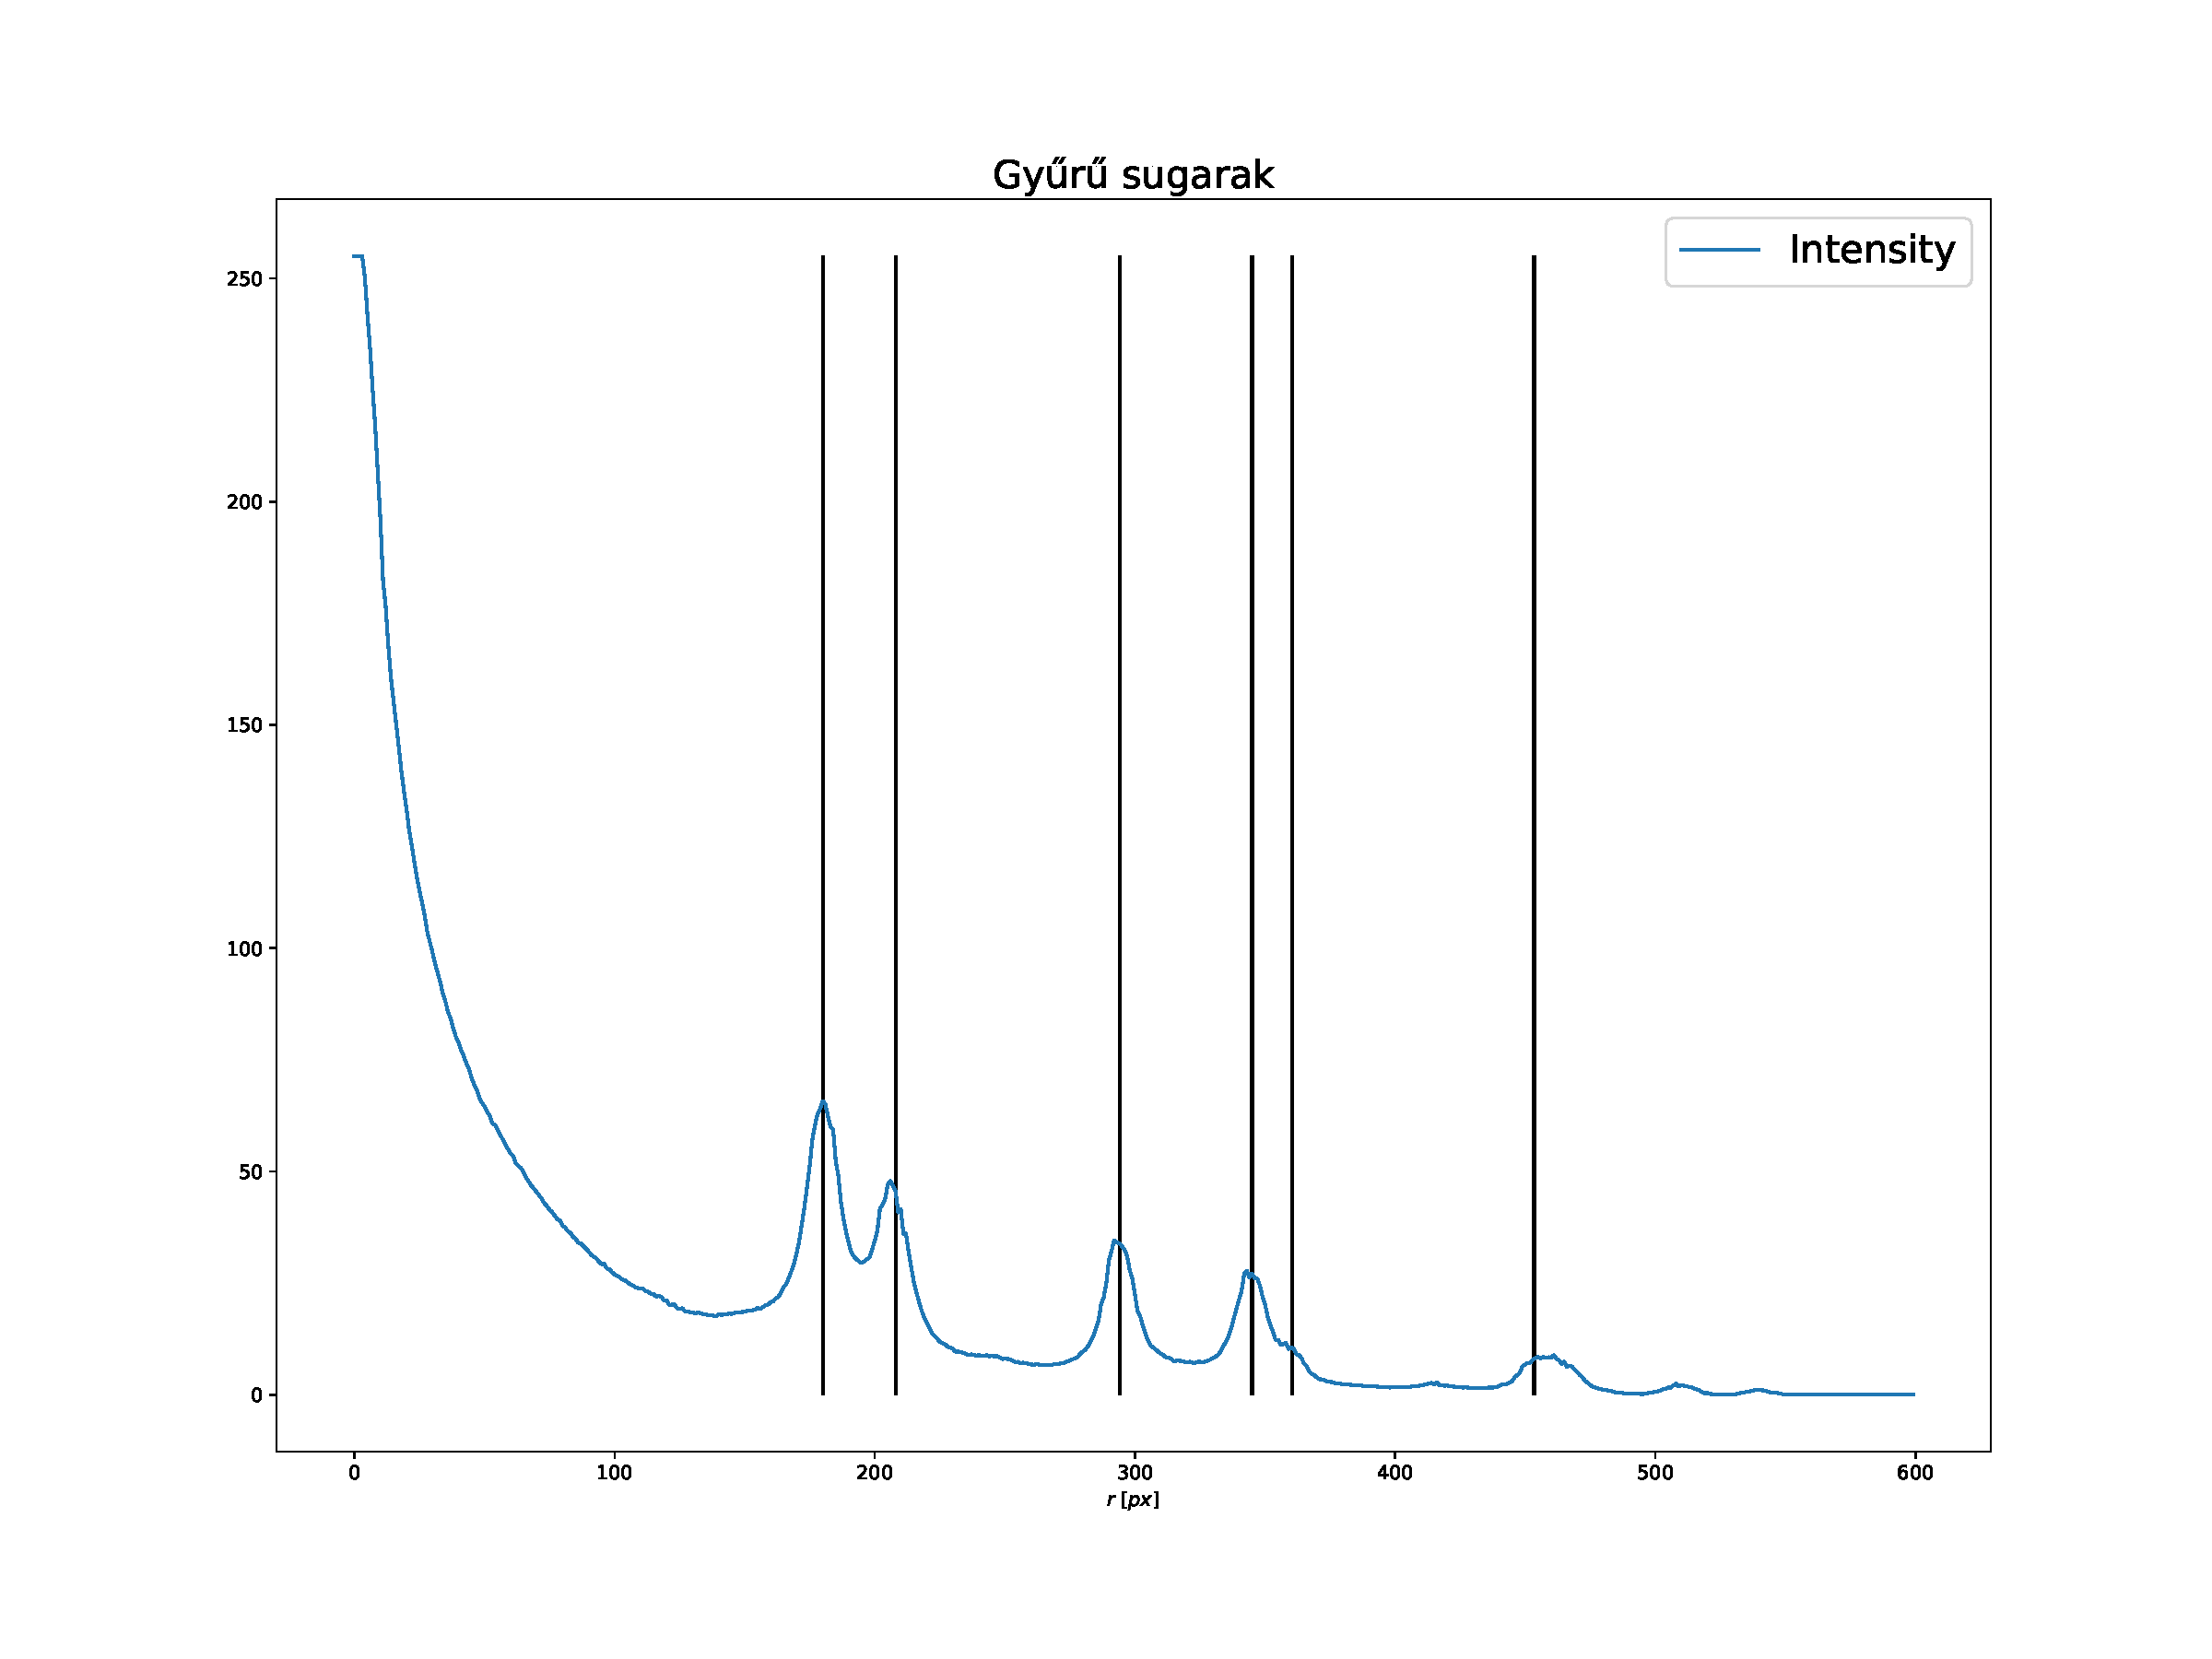
\includegraphics[scale=0.4]{sugarak.pdf}
			\caption{A középponttól mért távolság függvényében az átlagos intenzitás a körgyűrű mentén, illetve az illesztett mikroszkóp állandó által meghatározott gyűrű sugarak.}
			\label{sugarak}
		\end{figure}
		\begin{figure}[H]
			\centering
			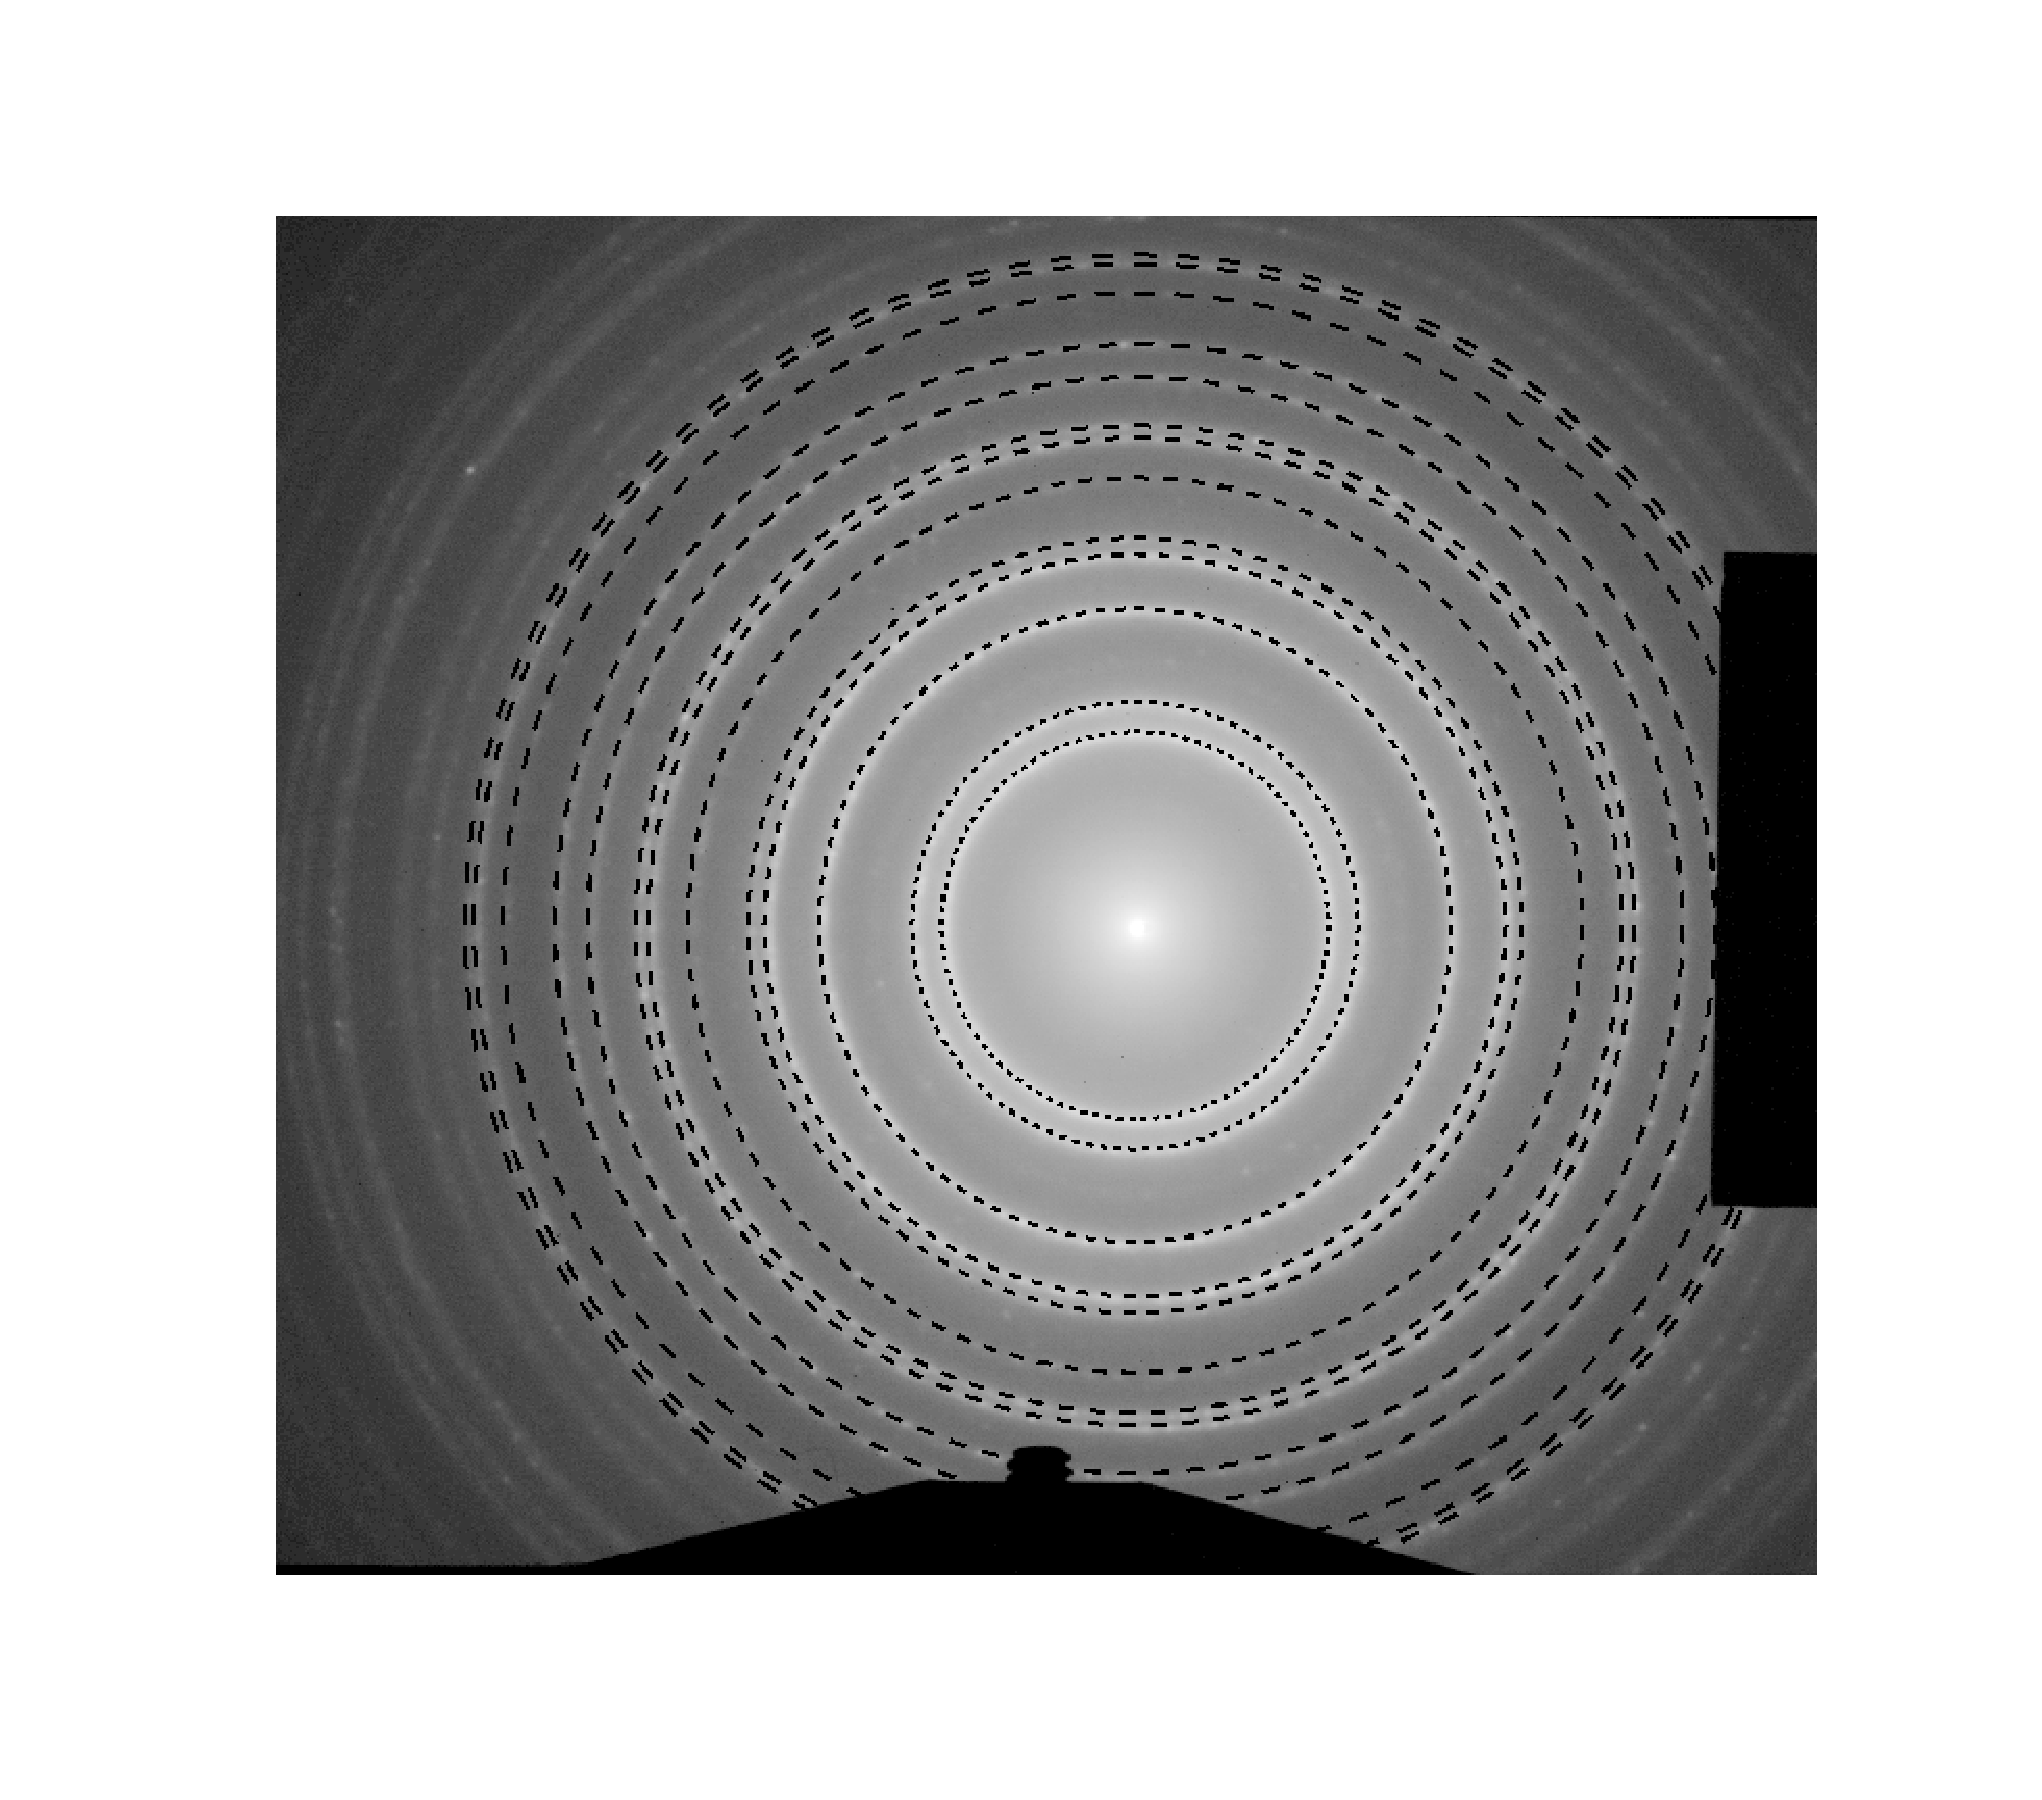
\includegraphics[scale=0.5]{gyuruk.pdf}
			\caption{A kalibrációs ábra az első néhány gyűrűvel az illesztett mikroszkóp állandónak megfelelően.}
			\label{gyuruk}
		\end{figure}
	\section{Szilícim}
		
		\begin{figure}[H]
			\centering
			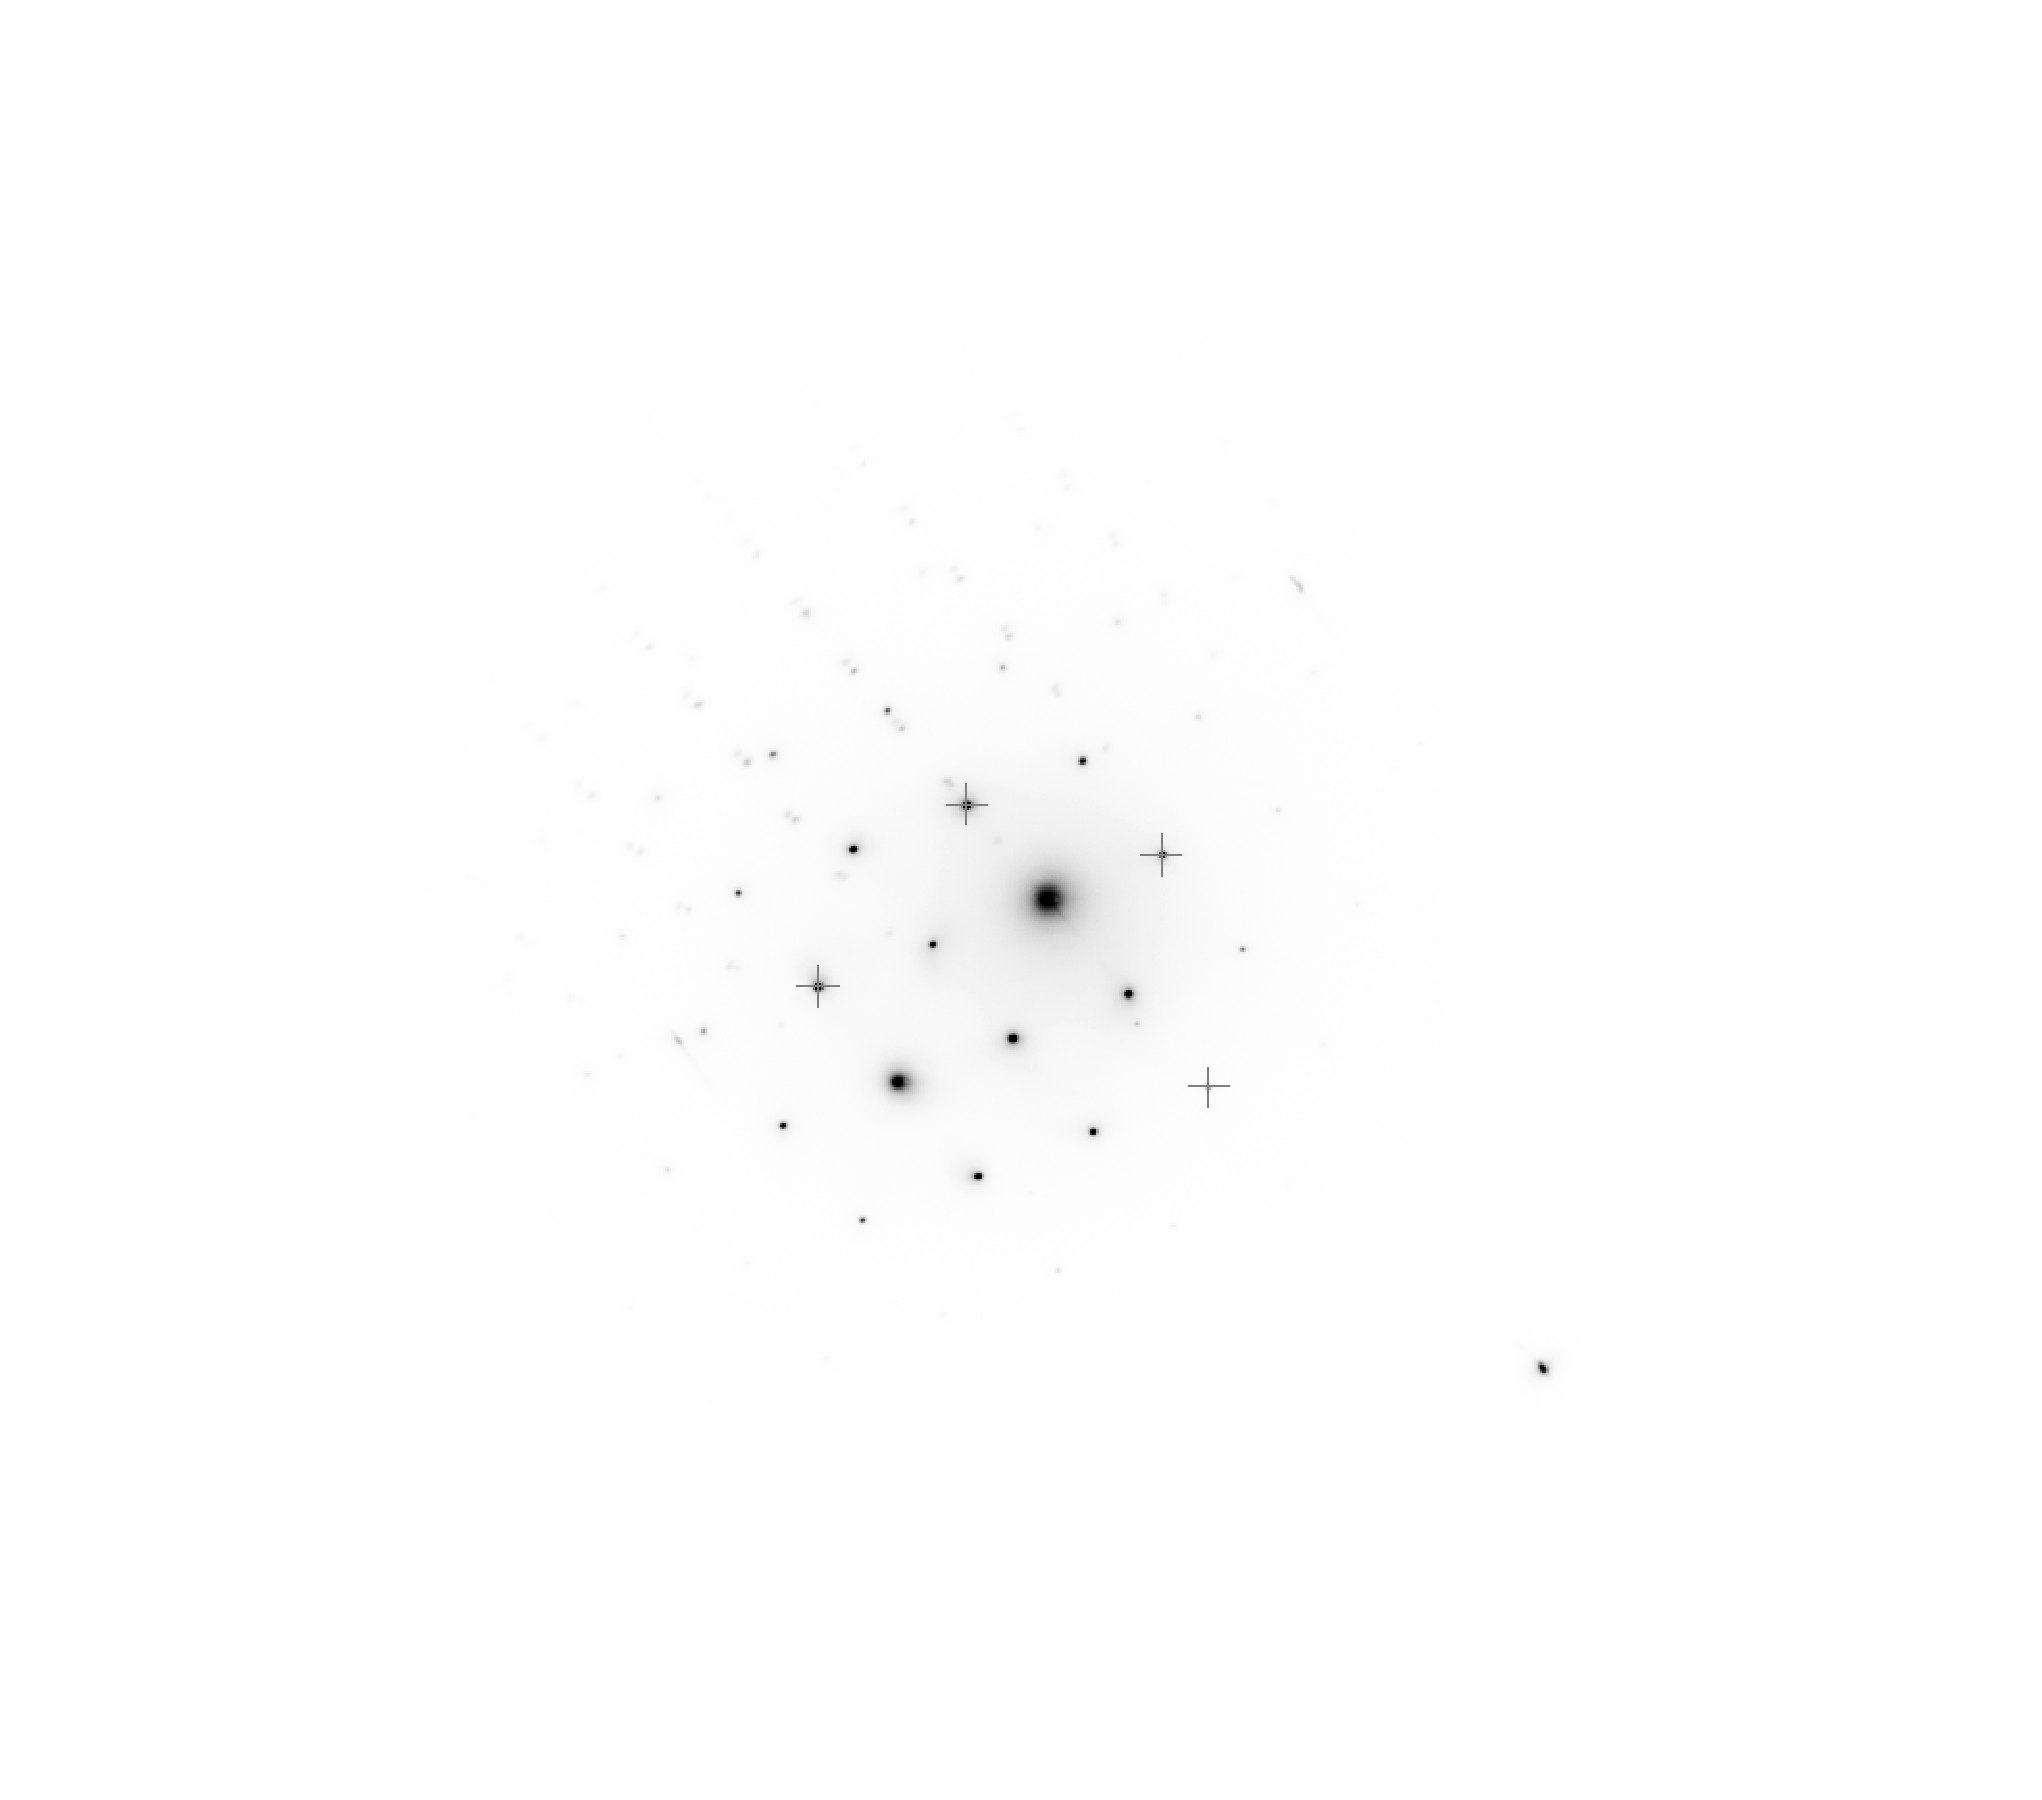
\includegraphics[scale=0.5]{si.pdf}
			\caption{A szilícium diffrakciós képe és a kiválasztott csúcsok. Föntről lefelé a diffrakciós csúcsok O, A, B és C.}
			\label{si}
		\end{figure}
		\begin{table}[H]
			\centering
			\begin{tabular}{|c|c|c|c|}
				\hline
				Csúcs & $R$ [pixel] & $d$ [\AA] & $(hkl)$\\
				\hline
				$OA$ & $187$ & $1.96$ & $(220)$\\
				$OB$ & $219$ & $1.68$ & $(1\bar{3}1)$\\
				$OC$ & $346$ & $1.06$ & $(511)$\\
				\hline
			\end{tabular}
			\caption{A szilícium diffrakciós ábra indexelése.}
		\end{table}
		\aref{si}. ábra szerinte a csúcsok közötti összefüggés $2OA+OB=OC$. Ellenőrzésképpen ezt kiszámítottam a csúcsok pozícióinak segítségével, és az összeg hibája $1.4\text{pixel}$ volt. A $(hkl)$ indexeket úgy választottam meg, hogy a vektoriális összefüggés teljesüljön. A mért $d$ értékek körülbelül $2\%$-kal nagyobbak voltak, mint a táblázatban talált értékek, ezért a mikroszkóp állandót korrigáltam ezzel az eltéréssel. A csúcsok alapján kapott mikroszkóp állandóban jobban bízom, mivel a középpont meghatározása a gyűrűk esetében nem volt teljesen pontos, a szilícium diffrakciós ábrája tisztábbnak látszik. A továbbiakban $\lambda L = 359\text{pixel\AA}$ értéket használtam, ezzel a szilícium esetében a számított és a táblázat beli $d$ értékek közötti eltérés $0.5\%$, $0.4\%$ illetve $0.1\%$ volt.
		
		A zónatengelyt $OB\times OA$ adja, az ábrából kifelé mutató irányban. $(1\bar{3}1)\times(220)=[\bar{2}28]\propto[\bar{1}14]$ a szilícium zónatengelye.
	\section{Gallium-nitrid}
		\begin{figure}[H]
			\centering
			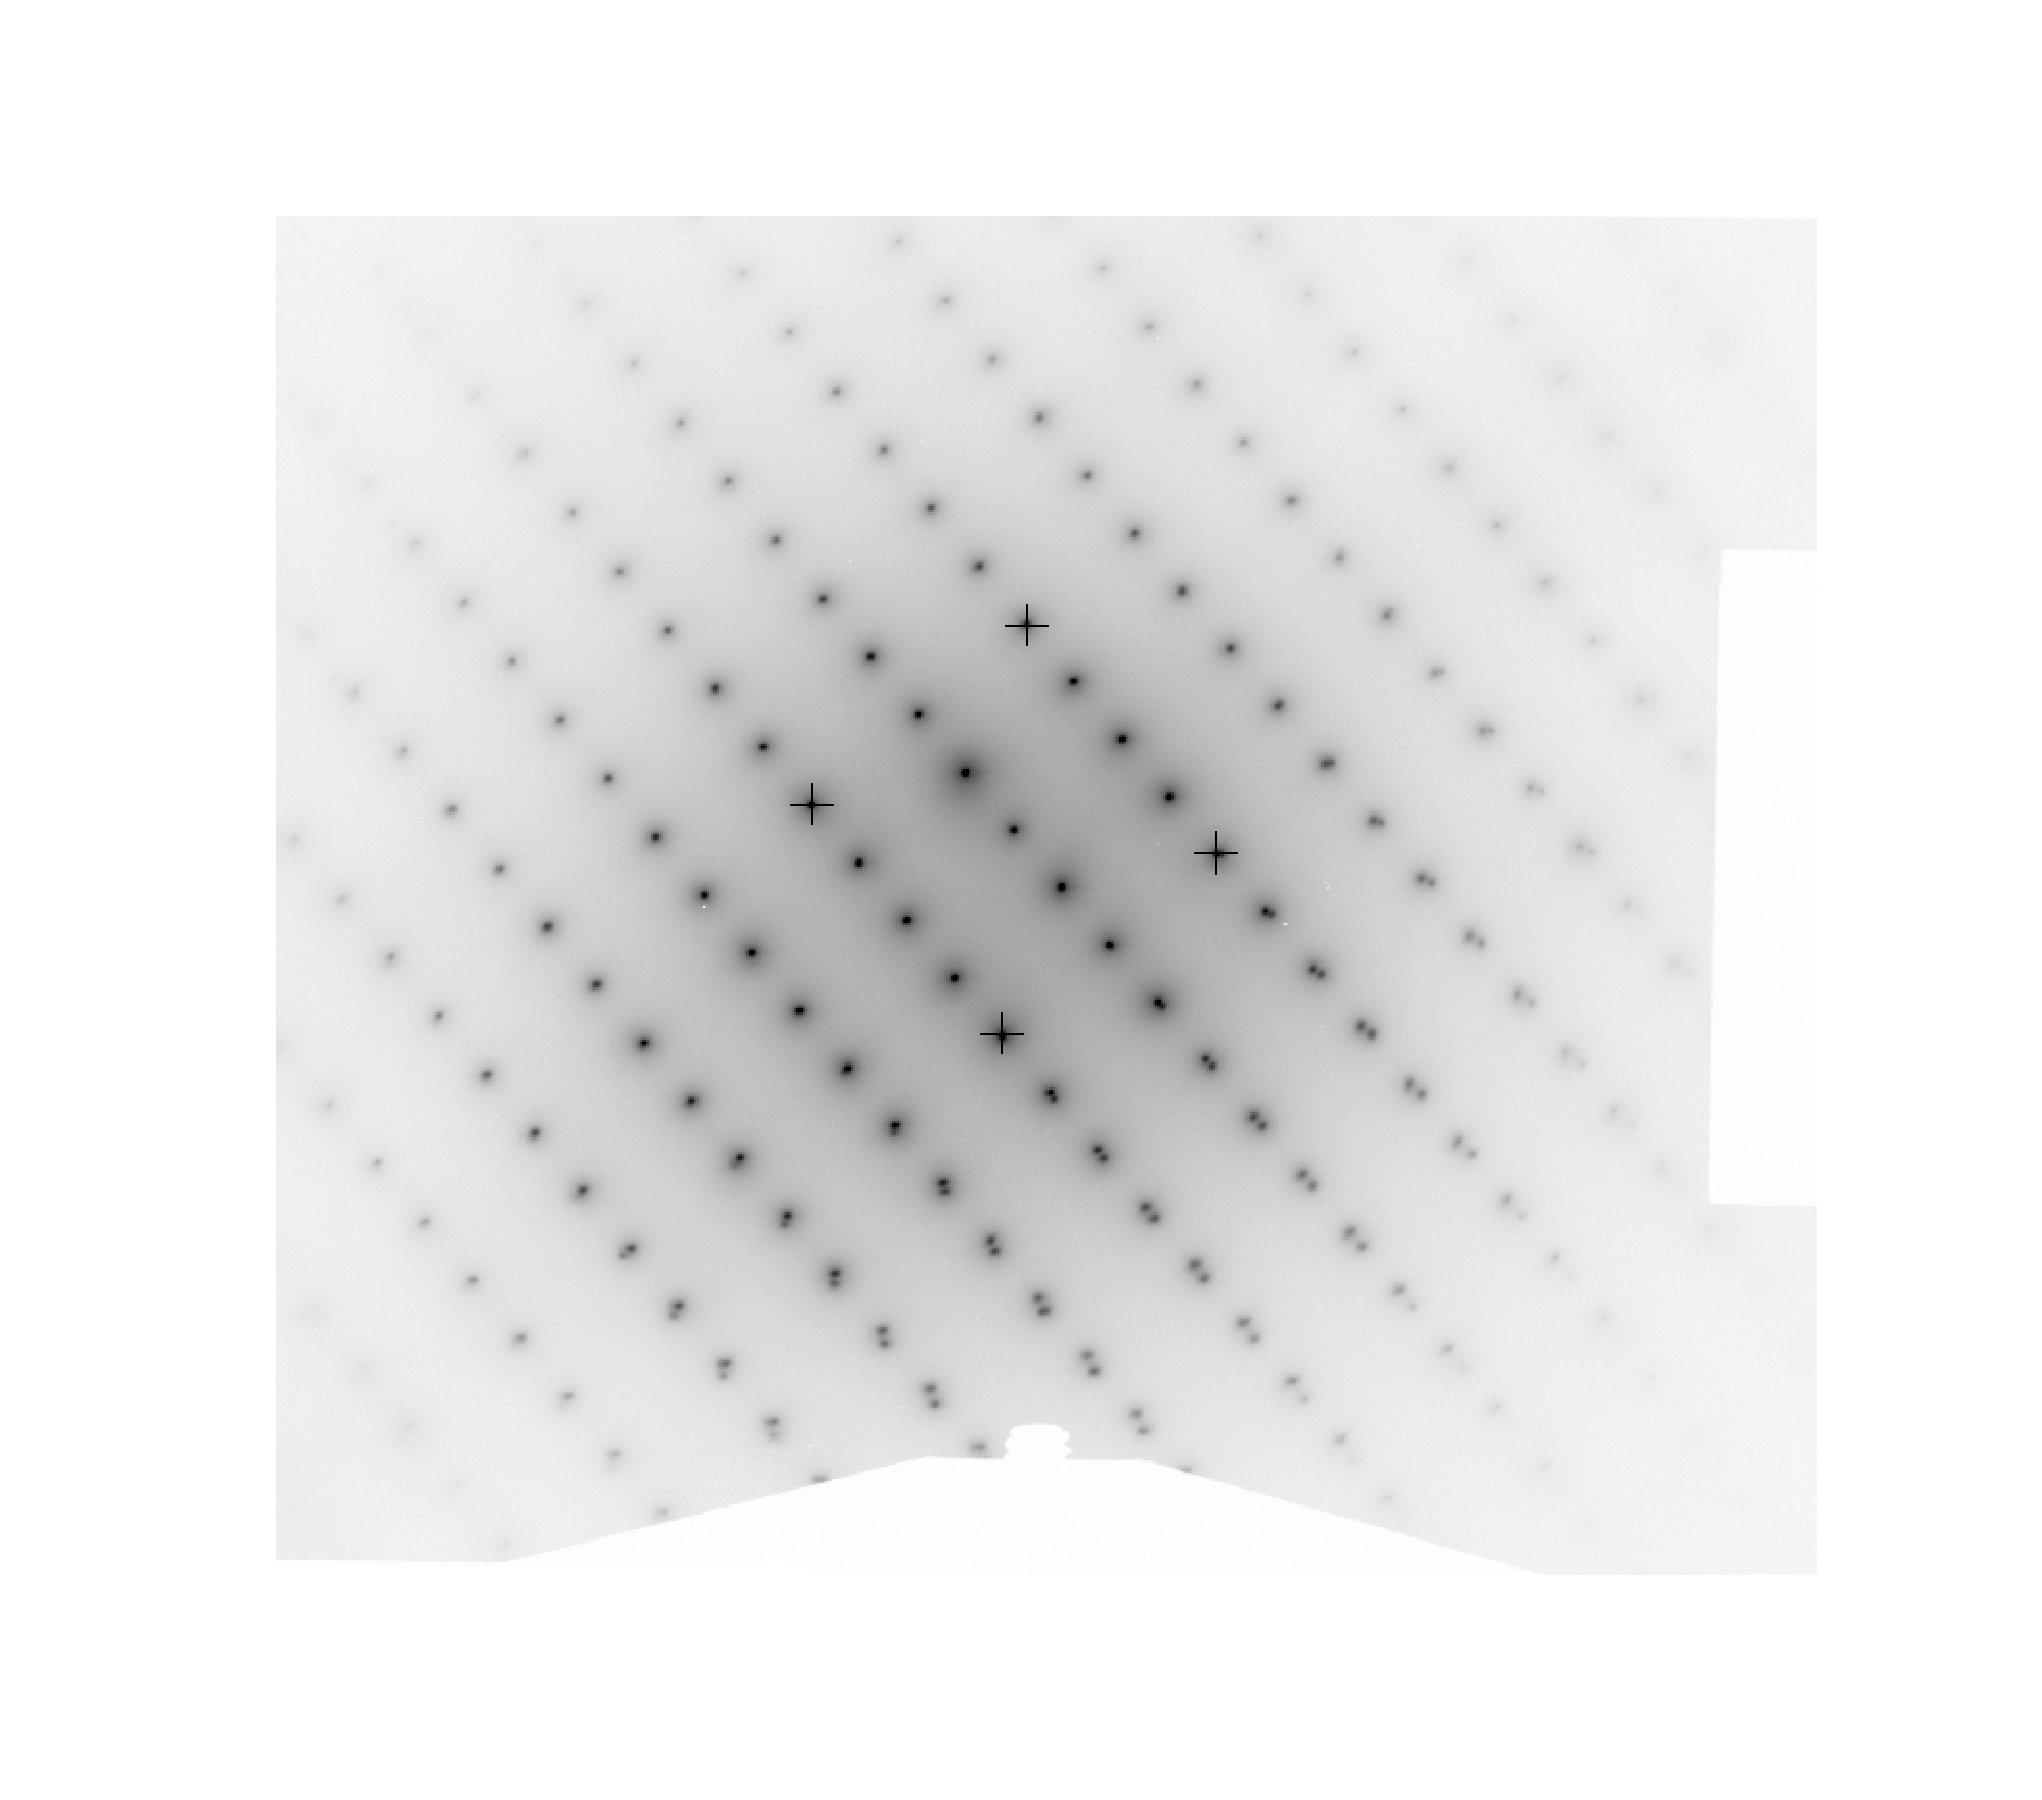
\includegraphics[scale=0.5]{gan.pdf}
			\caption{A gallium-nitrid diffrakciós képe és a kiválasztott csúcsok. Föntről lefelé a diffrakciós csúcsok O, A, B és C.}
			\label{gan}
		\end{figure}
		\begin{table}[H]
			\centering
			\begin{tabular}{|c|c|c|c|}
				\hline
				Csúcs & $R$ [pixel] & $d$ [\AA] & $(hkl)$\\
				\hline
				$OA$ & $260$ & $1.38$ & $(200)$\\
				$OB$ & $277$ & $1.30$ & $(004)$\\
				$OC$ & $381$ & $0.94$ & $(204)$\\
				\hline
			\end{tabular}
			\caption{A gallium-nitrid diffrakciós ábra indexelése.}
		\end{table}
		Az itt bejelölt csúcsokra vonatkozó egyenlet a $OA+OB=OC$. Ez teljesül $1.7\text{pixel}$ hibával. A Miller indexeket ennek az egyenletnek megfelelően választottam meg. A gallium-nitrid esetében a mért és a táblázatban felsorolt $d$ értékek közötti eltérés $0.4\%$ $0.1\%$ és $0.4\%$. Itt nem volt szükség rá, de hexagonális kristály esetében a $(200)$-val ekvivalens reciprokrács vektorok a négy indexes formalizmus segítségével kaphatóak meg, és ezek a $(\bar{2}020)$, $(\bar{2}200)$, $(2\bar{2}00)$, $(02\bar{2}0)$ valamint a $(0\bar{2}20)$ vektorok. Hasonlóak a $(204)$ vektorral ekvivalens vektorok, a $(004)$ vektorral pedig csak a $(00\bar{4})$ ekvivalens.
		
		A gallium-nitrid zónatengelyét előjel helyesen az $OA\times OB$ adja meg. $(200)\times (004)=[0\bar{8}0]\propto[0\bar{1}0]$ az elektronforrás felé mutató rácsvektor. A $[0\bar{1}00]$ négyes vektor nem teljesíti a $T=-(U+V)$ feltételt, viszont a zónatengelynek megfelelő irányát jelöli. Az $[1110]$ vektor a nullvektornak felel meg, tehát ennek a többszörösét hozzáadva a $[0\bar{1}00]$ vektor nem változik. $1/3$ szorzó választásával a négyes indexekre vonatkozó feltétel teljesül. Az eredményt megszoroztam 3-mal, hogy egész számokat kapjak. A végeredmény, hogy a zónatengely négy indexes jelölésben $[1\bar{2}10]$.
	\section{Közös kiértékelés}
		A vegyes diffrakciós ábra alapján a párhuzamos síkseregek a két anyagban az $(511)$ síksereg a szilícium esetében, a $\text{GaN}$ esetében pedig a $(001)$ síksereg. Ezekre a síkokra merőleges irányok párhuzamosak lesznek a két anyagban, azaz a szilícium $[511]$ és a gallium-nitrid $[001]$ irányai párhuzamosak. A szilícium köbös szerkezetű, a gallium-nitrid esetében pedig a kérdéses síkokat a $c^*$ reciprok vektor határozza meg, mellyel a $c$ rácsvektor párhuzamos, így mind a két esetben a síkokra merőleges irányok meghatározása könnyű volt.
		
		A zónatengely és a közös síkokra merőleges irány valóban merőleges a szilícium és gallium-nitrid esetében is. Ennek oka, hogy definíció szerint a zónatengelyhez tartozó síkok párhuzamosak a zónatengellyel. Ezek közül a síkseregek közül az egyik okozza mind a két mintában a közös egyenesbe eső diffrakciós pontokat. A közös irány ezekre a síkokra merőleges, így a zónatengelyre is.
		
		A reciprok vektorok amik merőlegesek a két közös irányra vektoriális szorzással megkaphatóak. A szilícium esetében $[511]\times[\bar{1}14]=(3,\bar{21},4)$, a gallium-nitrid esetében $[001]\times[0\bar{1}0]=(100)$ a reciprok vektor indexei.
	\bibliographystyle{abeld}
    %\bibliography{ref}
\end{document}